\documentclass[a4paper,12pt]{article}
\usepackage[utf8]{inputenc}
\usepackage{graphicx}
\usepackage{float}
\usepackage[spanish]{babel}
\usepackage{listings}
\usepackage{xcolor}
\usepackage{courier}
\usepackage[T1]{fontenc}

\definecolor{gris}{RGB}{123, 126, 132}
\definecolor{morado}{RGB}{81, 40, 155}
\definecolor{amarillo}{RGB}{253,151,31}
\definecolor{magenta}{RGB}{249,38,114}

\renewcommand{\lstlistingname}{Archivo}

\lstdefinestyle{customJava}{
    frame=tb,
    language=Java,
    backgroundcolor=\color{white},   
    commentstyle=\itshape\color{gris},
    keywordstyle=\bfseries\color{magenta},
    numberstyle=\color{morado},
    stringstyle=\color{amarillo},
    identifierstyle=\color{black},
    basicstyle=\footnotesize,
    breakatwhitespace=false,         
    breaklines=true,                 
    captionpos=b,
    keepspaces=true,                 
    numbers=left,                    
    numbersep=5pt,                  
    showspaces=false,                
    showstringspaces=false,
    showtabs=false,                  
    tabsize=2,
}

\lstdefinestyle{customXML}{
    frame=tb,
    language=XML,
    backgroundcolor=\color{white},   
    commentstyle=\itshape\color{gris},
    keywordstyle=\bfseries\color{magenta},
    numberstyle=\color{morado},
    stringstyle=\color{amarillo},
    identifierstyle=\color{black},
    basicstyle=\footnotesize,
    breakatwhitespace=false,         
    breaklines=true,                 
    captionpos=b,
    keepspaces=true,                 
    numbers=left,                    
    numbersep=5pt,                  
    showspaces=false,                
    showstringspaces=false,
    showtabs=false,                  
    tabsize=2,
}

%opening
\title{Ejercicio No. 4. Instituto (JSP, Gráficas y Login)}
\author{Barrera Pérez Carlos Tonatihu \\ Profesor: José Asunción Enríquez 
Zárate \\ Web Application Development \\ Grupo: 3CM9 }


\begin{document}

\maketitle

\newpage
\tableofcontents
\newpage
\section{Introducción}
Este ejercicio tuvo como objetivo modificar el ejercicio 3 y en lugar de 
utilizar solo servelts, utilizar JSPs para la vista, es importante señalar que 
la base de datos se modifico ya que ahora también se incluye la funcionalidad 
de inicio se sesión y se tienen perfiles de profesor y alumno, la base de datos 
final es la que se muestra en la figura \ref{fig:bd}.

\begin{figure}[H]
\begin{center}
 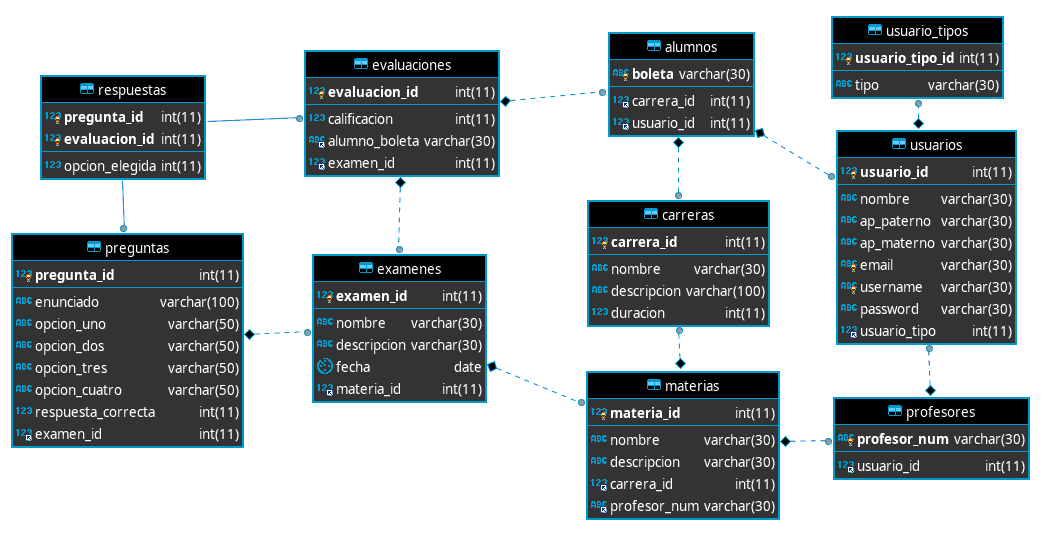
\includegraphics[width=\textwidth]{base.png}
 \caption{Base de datos que se trabajo en MySQL}
 \label{fig:bd}
\end{center}
\end{figure}

Otra funcionalidad que se le agrego es la generación de gráfica de cantidad de 
alumnos por carrera, así como el envió de dicha imagen al correo del usuario 
cuya sesión se encuentre activa y también se manda un correo si se requiere 
recuperar la contraseña.

Finalmente, se utiliza un filtro para manejar la autenticación de los usuarios 
y poder controlar las sesiones.

\section{Desarrollo}

\subsection{Código}

\begin{lstlisting}[language=Java, style=customJava, 
caption={EnvioEmail.java}, captionpos=b,basicstyle=\fontfamily{cmss}\small]
package utils;

import java.util.Map;
import java.util.Properties;
import java.util.logging.Level;
import java.util.logging.Logger;
import javax.activation.DataHandler;
import javax.activation.DataSource;
import javax.activation.FileDataSource;
import javax.mail.Authenticator;
import javax.mail.BodyPart;
import javax.mail.Message;
import javax.mail.MessagingException;
import javax.mail.PasswordAuthentication;
import javax.mail.Session;
import javax.mail.Transport;
import javax.mail.internet.AddressException;
import javax.mail.internet.InternetAddress;
import javax.mail.internet.MimeBodyPart;
import javax.mail.internet.MimeMessage;
import javax.mail.internet.MimeMultipart;

/**
 *
 * @author tonatihu
 * Created on 10-Mar-2019
 */
public class EnvioEmail {
    private String asunto;
    private String destinatario;
    private String mensaje;
    private Properties props;
    private static final String USERNAME = "webappdevtona@outlook.com";
    private static final String PASSWORD = "jodanse90";
    private final Session session;
    
    public EnvioEmail() {
        props = new Properties();
        props.put("mail.smtp.auth", "true");
        props.put("mail.smtp.starttls.enable", "true");
        props.put("mail.smtp.host", "smtp.office365.com");
        props.put("mail.smtp.port", "587");
        session = Session.getInstance(props, new Authenticator() {
            @Override
            protected PasswordAuthentication getPasswordAuthentication() {
                return new PasswordAuthentication(USERNAME, PASSWORD);
            }
        });
    }

    public String getAsunto() {
        return asunto;
    }

    public void setAsunto(String asunto) {
        this.asunto = asunto;
    }

    public String getDestinatario() {
        return destinatario;
    }

    public void setDestinatario(String destinatario) {
        this.destinatario = destinatario;
    }

    public String getMensaje() {
        return mensaje;
    }

    public void setMensaje(String mensaje) {
        this.mensaje = mensaje;
    }
    
    public void enviar(Map<String, String> imagenes, Map<String, String> 
archivos) {
        try {
            Message message = new MimeMessage(session);
            message.setFrom(new InternetAddress(USERNAME));
            message.setRecipients(Message.RecipientType.TO, 
InternetAddress.parse(destinatario));
            message.setSubject(asunto);
            
            MimeMultipart multipart = new MimeMultipart("related");
            
            BodyPart bodyPartMensaje = new MimeBodyPart();
            bodyPartMensaje.setContent(mensaje, "text/html;charset=UTF-8");
            multipart.addBodyPart(bodyPartMensaje);
            
            for (Map.Entry<String, String> entrada : imagenes.entrySet()) {
                BodyPart bodyPartImagenes = new MimeBodyPart();
                DataSource fds = new FileDataSource(entrada.getValue());
                bodyPartImagenes.setDataHandler(new DataHandler(fds));
                bodyPartImagenes.setHeader("Content-ID", "<" + entrada.getKey() 
+ ">");
                multipart.addBodyPart(bodyPartImagenes);
            }
            
            for (Map.Entry<String, String> entrada : archivos.entrySet()) {
                BodyPart bodyPartArchivos = new MimeBodyPart();
                DataSource fds2 = new FileDataSource(entrada.getValue());
                bodyPartArchivos.setDataHandler(new DataHandler(fds2));
                bodyPartArchivos.setFileName(entrada.getKey());
                multipart.addBodyPart(bodyPartArchivos);
            }
            
            message.setContent(multipart);
            
            Transport.send(message);
        } catch (AddressException ex) {
            Logger.getLogger(EnvioEmail.class.getName()).log(Level.SEVERE, 
"Error AddressException", ex);
        } catch (MessagingException ex) {
            Logger.getLogger(EnvioEmail.class.getName()).log(Level.SEVERE, 
"Error MessagingException", ex);
        }
    }
}

\end{lstlisting}

\begin{lstlisting}[language=Java, style=customJava, 
caption={RecuperarContraServlet.java},captionpos=b,basicstyle=\fontfamily{cmss}
\small]
package controller;

import dao.UsuarioDao;
import dao.impl.UsuarioDaoImpl;
import dto.Usuario;
import java.io.IOException;
import java.sql.SQLException;
import java.util.HashMap;
import java.util.Map;
import java.util.logging.Level;
import java.util.logging.Logger;
import javax.servlet.ServletException;
import javax.servlet.annotation.WebServlet;
import javax.servlet.http.HttpServlet;
import javax.servlet.http.HttpServletRequest;
import javax.servlet.http.HttpServletResponse;
import utils.EnvioEmail;

/**
 *
 * @author tonatihu
 * Created on 09-Mar-2019
 */
@WebServlet(name="ForgotPassword", urlPatterns={"/forgotPassword"})
public class RecuperarContraServlet extends HttpServlet {
   
    /** 
     * Processes requests for both HTTP <code>GET</code> and <code>POST</code> 
methods.
     * @param request servlet request
     * @param response servlet response
     * @throws ServletException if a servlet-specific error occurs
     * @throws IOException if an I/O error occurs
     */
    protected void processRequest(HttpServletRequest request, 
HttpServletResponse response)
    throws ServletException, IOException {
        request.setCharacterEncoding("UTF-8");
        String email = request.getParameter("email");
        UsuarioDao dao = new UsuarioDaoImpl();
        Map<String, String> imagenesMap = new HashMap<>();
        Map<String, String> archivosMap = new HashMap<>();
        
        if (email != null) {
            try {
                EnvioEmail e = new EnvioEmail();
                e.setAsunto("Recuperar contrasena de Instituto");
                e.setDestinatario(email);
                Usuario u = dao.findByEmail(email);
                if (u != null) {
                    String mensaje = "<h1>Bienvenido a Instituto</h1><br><h2>Tu 
contrasena es:</h2> " 
                            + u.getPassword();
                    e.setMensaje(mensaje);
                    e.enviar(imagenesMap, archivosMap);
                    response.sendRedirect("login");
                    return;
                }
            } catch (SQLException ex) {
                
Logger.getLogger(RecuperarContraServlet.class.getName()).log(Level.SEVERE, null, 
ex);
            }
            
        }
        request.getRequestDispatcher("forgotPassword.jsp").forward(request, 
response);
    } 

    // <editor-fold defaultstate="collapsed" desc="HttpServlet methods. Click on 
the + sign on the left to edit the code.">
    /** 
     * Handles the HTTP <code>GET</code> method.
     * @param request servlet request
     * @param response servlet response
     * @throws ServletException if a servlet-specific error occurs
     * @throws IOException if an I/O error occurs
     */
    @Override
    protected void doGet(HttpServletRequest request, HttpServletResponse 
response)
    throws ServletException, IOException {
        processRequest(request, response);
    } 

    /** 
     * Handles the HTTP <code>POST</code> method.
     * @param request servlet request
     * @param response servlet response
     * @throws ServletException if a servlet-specific error occurs
     * @throws IOException if an I/O error occurs
     */
    @Override
    protected void doPost(HttpServletRequest request, HttpServletResponse 
response)
    throws ServletException, IOException {
        processRequest(request, response);
    }

    /** 
     * Returns a short description of the servlet.
     * @return a String containing servlet description
     */
    @Override
    public String getServletInfo() {
        return "Short description";
    }// </editor-fold>

}
\end{lstlisting}

\begin{lstlisting}[language=Java, style=customJava, 
caption={GraficasServlet.java}, captionpos=b,basicstyle=\fontfamily{cmss}\small]
package controller;

import dao.AlumnoDao;
import dao.impl.AlumnoDaoImpl;
import dto.Datos;
import dto.Usuario;
import java.io.File;
import java.io.IOException;
import java.sql.SQLException;
import java.util.HashMap;
import java.util.List;
import java.util.Map;
import java.util.logging.Level;
import java.util.logging.Logger;
import javax.servlet.ServletException;
import javax.servlet.annotation.WebServlet;
import javax.servlet.http.HttpServlet;
import javax.servlet.http.HttpServletRequest;
import javax.servlet.http.HttpServletResponse;
import javax.servlet.http.HttpSession;
import org.jfree.chart.ChartFactory;
import org.jfree.chart.ChartUtilities;
import org.jfree.chart.JFreeChart;
import org.jfree.data.general.DefaultPieDataset;
import utils.EnvioEmail;
import utils.Paginas;

/**
 *
 * @author tonatihu
 * Created on 10-Mar-2019
 */
@WebServlet(name="GraficasServlet", urlPatterns={"/graficas"})
public class GraficasServlet extends HttpServlet {
     private static final Logger LOGGER = 
Logger.getLogger(GraficasServlet.class.getName());
   
    /** 
     * Processes requests for both HTTP <code>GET</code> and <code>POST</code> 
methods.
     * @param request servlet request
     * @param response servlet response
     * @throws ServletException if a servlet-specific error occurs
     * @throws IOException if an I/O error occurs
     */
    protected void processRequest(HttpServletRequest request, 
HttpServletResponse response)
    throws ServletException, IOException {
        response.setContentType("text/html;charset=UTF-8");
        request.setCharacterEncoding("UTF-8");
        String accion = request.getParameter("action");
        if (accion.equals("ver"))
            ver(request, response);
        else if (accion.equals("generar"))
            enviar(request, response);
    } 

    // <editor-fold defaultstate="collapsed" desc="HttpServlet methods. Click on 
the + sign on the left to edit the code.">
    /** 
     * Handles the HTTP <code>GET</code> method.
     * @param request servlet request
     * @param response servlet response
     * @throws ServletException if a servlet-specific error occurs
     * @throws IOException if an I/O error occurs
     */
    @Override
    protected void doGet(HttpServletRequest request, HttpServletResponse 
response)
    throws ServletException, IOException {
        processRequest(request, response);
    } 

    /** 
     * Handles the HTTP <code>POST</code> method.
     * @param request servlet request
     * @param response servlet response
     * @throws ServletException if a servlet-specific error occurs
     * @throws IOException if an I/O error occurs
     */
    @Override
    protected void doPost(HttpServletRequest request, HttpServletResponse 
response)
    throws ServletException, IOException {
        processRequest(request, response);
    }

    /** 
     * Returns a short description of the servlet.
     * @return a String containing servlet description
     */
    @Override
    public String getServletInfo() {
        return "Short description";
    }// </editor-fold>

    private void generarGrafica(List<Datos> datos) throws IOException {
        DefaultPieDataset dpd = new DefaultPieDataset();
        datos.forEach((d) -> {
            dpd.setValue(d.getNombre(), d.getCantidad());
        });
        String archivo = 
getServletConfig().getServletContext().getRealPath("/static/img/grafica.png");
        JFreeChart chart = ChartFactory.createPieChart("Cantidad de alumnos por 
carrera", 
               dpd, true, true, false);
        ChartUtilities.saveChartAsPNG(new File(archivo), chart, 400, 300);
    }

    private void ver(HttpServletRequest request, HttpServletResponse response) 
            throws IOException, ServletException, ServletException {
        try {
            request.setAttribute("PAGINA", Paginas.GRAFICAS);
            AlumnoDao dao = new AlumnoDaoImpl();
            List<Datos> datos = dao.getData();
            request.setAttribute("lista", datos);
            generarGrafica(datos);
            request.getRequestDispatcher("graficas.jsp").forward(request, 
response);
        } catch (SQLException ex) {
            Logger.getLogger(GraficasServlet.class.getName()).log(Level.SEVERE, 
null, ex);
        }
    }

    private void enviar(HttpServletRequest request, HttpServletResponse 
response) throws IOException {
        HttpSession session = request.getSession();
        Usuario u = (Usuario) session.getAttribute("USUARIO_SESSION");
        EnvioEmail e = new EnvioEmail();
        e.setAsunto("Envio de la cantidad de alumnos");
        e.setDestinatario(u.getEmail());
        String archivo = 
getServletConfig().getServletContext().getRealPath("/static/img/grafica.png");
        Map<String, String> imagenesMap = new HashMap<>();
        Map<String, String> archivosMap = new HashMap<>();
        imagenesMap.put("grafica", archivo);
        String mensaje = "<h1>Bienvenido a Instituto</h1><br><h2>Te mandamos una 
grafica bien chida</h2> <img src=\"cid:grafica\"/> ";
        e.setMensaje(mensaje);
        e.enviar(imagenesMap, archivosMap);
        response.sendRedirect("graficas?action=ver");
    }
}

\end{lstlisting}

\begin{lstlisting}[language=Java, style=customJava, 
caption={AuthenticationFilter.java},captionpos=b,basicstyle=\fontfamily{cmss}
\small]
package interceptor;

import java.io.IOException;
import java.io.PrintWriter;
import java.io.StringWriter;
import javax.servlet.Filter;
import javax.servlet.FilterChain;
import javax.servlet.FilterConfig;
import javax.servlet.ServletException;
import javax.servlet.ServletRequest;
import javax.servlet.ServletResponse;
import javax.servlet.annotation.WebFilter;
import javax.servlet.http.HttpServletRequest;
import javax.servlet.http.HttpServletResponse;
import javax.servlet.http.HttpSession;

/**
 *
 * @author tonatihu
 */
@WebFilter(filterName = "AuthenticationFilter", urlPatterns = {"/*"})
public class AuthenticationFilter implements Filter {
    
    private static final boolean DEBUG = true;
    private FilterConfig filterConfig = null;
    
    public AuthenticationFilter() {
    }
    private static final String[] NO_REQUIERE_LOGIN = {
            "/static", "/login", "/signup", "forgotPassword",
    };
    
    private void doBeforeProcessing(ServletRequest request, ServletResponse 
response)
            throws IOException, ServletException {
        if (DEBUG) {
            log("AuthenticationFilter:DoBeforeProcessing");
        }
    }    
    
    private void doAfterProcessing(ServletRequest request, ServletResponse 
response)
            throws IOException, ServletException {
        if (DEBUG) {
            log("AuthenticationFilter:DoAfterProcessing");
        }
    }
    
    @Override
    public void doFilter(ServletRequest req, ServletResponse resp, 
            FilterChain chain) throws IOException, ServletException {
        if (DEBUG) {
            log("AuthenticationFilter:doFilter()");
        }
        doBeforeProcessing(req, resp);
        
        HttpServletRequest request = (HttpServletRequest) req;
        request.setCharacterEncoding("UTF-8");
        HttpServletResponse response = (HttpServletResponse) resp;
        HttpSession session = request.getSession(false);

        boolean isLoggedIn = (session != null && 
session.getAttribute("USUARIO_SESSION") != null);

        String url = request.getRequestURI();
        String logout = request.getParameter("logout");
        if (isLoggedIn && url.equals("/instituto/login") && logout == null) {
            if (DEBUG)
                log("Ya inicio sesion pero quiere hacerlo otra vez");
            response.sendRedirect("home");
        }else if(isLoggedIn || url.equals("/instituto/login") || 
loginRequerido(request)) {
            if (DEBUG)
                log("Quiere acceder a cualquier pagina o al login");
            chain.doFilter(req, resp);
        } else {
            if (DEBUG)
                log("No inicio sesion y se salta el login");
            response.sendRedirect("login");
        }
        
        doAfterProcessing(req, resp);
    }
    
    private boolean loginRequerido(HttpServletRequest request) {
        String requestURL = request.getRequestURL().toString();
        for (String url : NO_REQUIERE_LOGIN) {
            if (requestURL.contains(url))
                return true;
        }
        return false;
    }

    public FilterConfig getFilterConfig() {
        return (this.filterConfig);
    }

    public void setFilterConfig(FilterConfig filterConfig) {
        this.filterConfig = filterConfig;
    }

    @Override
    public void destroy() {        
    }

    @Override
    public void init(FilterConfig filterConfig) {        
        this.filterConfig = filterConfig;
        if (filterConfig != null) {
            if (DEBUG) {                
                log("AuthenticationFilter:Initializing filter");
            }
        }
    }

    @Override
    public String toString() {
        if (filterConfig == null) {
            return ("AuthenticationFilter()");
        }
        StringBuilder sb = new StringBuilder("AuthenticationFilter(");
        sb.append(filterConfig);
        sb.append(")");
        return (sb.toString());
    }
    
    public static String getStackTrace(Throwable t) {
        String stackTrace = null;
        try {
            StringWriter sw = new StringWriter();
            PrintWriter pw = new PrintWriter(sw);
            t.printStackTrace(pw);
            pw.close();
            sw.close();
            stackTrace = sw.getBuffer().toString();
        } catch (IOException ex) {
        }
        return stackTrace;
    }
    
    public void log(String msg) {
        filterConfig.getServletContext().log(msg);        
    }
    
}
\end{lstlisting}

\begin{lstlisting}[language=Java, style=customJava, 
caption={AlumnosServlet.java}, captionpos=b,basicstyle=\fontfamily{cmss}\small]
package controller;

import dao.AlumnoDao;
import dao.CarreraDao;
import dao.UsuarioDao;
import dao.impl.AlumnoDaoImpl;
import dao.impl.CarreraDaoImpl;
import dao.impl.UsuarioDaoImpl;
import dto.Alumno;
import dto.Usuario;
import java.io.IOException;
import java.sql.SQLException;
import java.util.List;
import java.util.logging.Level;
import java.util.logging.Logger;
import javax.servlet.ServletException;
import javax.servlet.annotation.WebServlet;
import javax.servlet.http.HttpServlet;
import javax.servlet.http.HttpServletRequest;
import javax.servlet.http.HttpServletResponse;

/**
 *
 * @author tonatihu
 * Created on 10-Mar-2019
 */
@WebServlet(name="AlumnosServlet", urlPatterns={"/alumnos"})
public class AlumnosServlet extends HttpServlet {
   
    /** 
     * Processes requests for both HTTP <code>GET</code> and <code>POST</code> 
methods.
     * @param request servlet request
     * @param response servlet response
     * @throws ServletException if a servlet-specific error occurs
     * @throws IOException if an I/O error occurs
     */
    protected void processRequest(HttpServletRequest request, 
HttpServletResponse response)
    throws ServletException, IOException {
        response.setContentType("text/html;charset=UTF-8");
        request.setCharacterEncoding("UTF-8");
        String action = request.getParameter("action");
        if (action.equals("ver"))
            mostrarAlumnos(request, response);
        else if (action.equals("eliminar"))
            eliminarAlumno(request, response);
        
    } 

    // <editor-fold defaultstate="collapsed" desc="HttpServlet methods. Click on 
the + sign on the left to edit the code.">
    /** 
     * Handles the HTTP <code>GET</code> method.
     * @param request servlet request
     * @param response servlet response
     * @throws ServletException if a servlet-specific error occurs
     * @throws IOException if an I/O error occurs
     */
    @Override
    protected void doGet(HttpServletRequest request, HttpServletResponse 
response)
    throws ServletException, IOException {
        processRequest(request, response);
    } 

    /** 
     * Handles the HTTP <code>POST</code> method.
     * @param request servlet request
     * @param response servlet response
     * @throws ServletException if a servlet-specific error occurs
     * @throws IOException if an I/O error occurs
     */
    @Override
    protected void doPost(HttpServletRequest request, HttpServletResponse 
response)
    throws ServletException, IOException {
        processRequest(request, response);
    }

    /** 
     * Returns a short description of the servlet.
     * @return a String containing servlet description
     */
    @Override
    public String getServletInfo() {
        return "Short description";
    }// </editor-fold>

    private void mostrarAlumnos(HttpServletRequest request, HttpServletResponse 
response) 
            throws ServletException, IOException {
        try {
            request.setAttribute("PAGINA", 7);
            AlumnoDao dao = new AlumnoDaoImpl();
            CarreraDao daoCarrera = new CarreraDaoImpl();
            List<Alumno> alumnos = dao.readAll();
            for (Alumno alumno : alumnos) {
                alumno.setCarrera(daoCarrera.read(alumno.getCarrera()));
            }
            request.setAttribute("alumnos", alumnos);
            request.getRequestDispatcher("listaAlumnos.jsp").forward(request, 
response);
        } catch (SQLException ex) {
            Logger.getLogger(AlumnosServlet.class.getName()).log(Level.SEVERE, 
null, ex);
        }
    }

    private void eliminarAlumno(HttpServletRequest request, HttpServletResponse 
response) 
            throws IOException {
        try {
            UsuarioDao dao = new UsuarioDaoImpl();
            int id = Integer.parseInt(request.getParameter("id"));
            Usuario usuario = new Usuario();
            usuario.setId(id);
            dao.delete(usuario);
            response.sendRedirect("alumnos?action=ver");
        } catch (SQLException ex) {
            Logger.getLogger(AlumnosServlet.class.getName()).log(Level.SEVERE, 
null, ex);
        }
    }

}
\end{lstlisting}

\begin{lstlisting}[language=Java, style=customJava, 
caption={CarrerasServlet.java}, captionpos=b,basicstyle=\fontfamily{cmss}\small]
package controller;

import dao.CarreraDao;
import dao.impl.CarreraDaoImpl;
import dto.Carrera;
import java.io.IOException;
import java.sql.SQLException;
import java.util.List;
import java.util.logging.Level;
import java.util.logging.Logger;
import javax.servlet.ServletException;
import javax.servlet.annotation.WebServlet;
import javax.servlet.http.HttpServlet;
import javax.servlet.http.HttpServletRequest;
import javax.servlet.http.HttpServletResponse;
import utils.Paginas;

/**
 *
 * @author tonatihu
 * Created on 10-Mar-2019
 */
@WebServlet(name="CarrerasServlet", urlPatterns={"/carreras"})
public class CarrerasServlet extends HttpServlet {
   
    /** 
     * Processes requests for both HTTP <code>GET</code> and <code>POST</code> 
methods.
     * @param request servlet request
     * @param response servlet response
     * @throws ServletException if a servlet-specific error occurs
     * @throws IOException if an I/O error occurs
     */
    protected void processRequest(HttpServletRequest request, 
HttpServletResponse response)
    throws ServletException, IOException {
        response.setContentType("text/html;charset=UTF-8");
        request.setCharacterEncoding("UTF-8");
        String action = request.getParameter("action");
        switch (action) {
            case "ver":
                verCarreras(request, response);
                break;
            case "eliminar":
                eliminarCarrera(request, response);
                break;
            case "editar":
                editarCarrera(request, response);
                break;
            case "agregar":
                agregarCarrera(request, response);
                break;
            case "guardar":
                guardarCarrera(request, response);
                break;
            default:
                response.sendRedirect("home");
                break;
        }
    } 

    // <editor-fold defaultstate="collapsed" desc="HttpServlet methods. Click on 
the + sign on the left to edit the code.">
    /** 
     * Handles the HTTP <code>GET</code> method.
     * @param request servlet request
     * @param response servlet response
     * @throws ServletException if a servlet-specific error occurs
     * @throws IOException if an I/O error occurs
     */
    @Override
    protected void doGet(HttpServletRequest request, HttpServletResponse 
response)
    throws ServletException, IOException {
        processRequest(request, response);
    } 

    /** 
     * Handles the HTTP <code>POST</code> method.
     * @param request servlet request
     * @param response servlet response
     * @throws ServletException if a servlet-specific error occurs
     * @throws IOException if an I/O error occurs
     */
    @Override
    protected void doPost(HttpServletRequest request, HttpServletResponse 
response)
    throws ServletException, IOException {
        processRequest(request, response);
    }

    /** 
     * Returns a short description of the servlet.
     * @return a String containing servlet description
     */
    @Override
    public String getServletInfo() {
        return "Short description";
    }// </editor-fold>

    private void verCarreras(HttpServletRequest request, HttpServletResponse 
response) 
            throws ServletException, IOException {
        try {
            request.setAttribute("PAGINA", Paginas.MOSTRAR_CARRERAS);
            CarreraDao dao = new CarreraDaoImpl();
            List<Carrera> carreras = dao.readAll();
            request.setAttribute("carreras", carreras);
            request.getRequestDispatcher("listaCarreras.jsp").forward(request, 
response);
        } catch (SQLException ex) {
            Logger.getLogger(CarrerasServlet.class.getName()).log(Level.SEVERE, 
null, ex);
        }
    }

    private void eliminarCarrera(HttpServletRequest request, HttpServletResponse 
response) {
        try {
            int id = Integer.valueOf(request.getParameter("id"));
            CarreraDao dao = new CarreraDaoImpl();
            Carrera c = new Carrera();
            c.setId(id);
            dao.delete(c);
            response.sendRedirect("carreras?action=ver");
        } catch (IOException | SQLException ex) {
            Logger.getLogger(CarrerasServlet.class.getName()).log(Level.SEVERE, 
null, ex);
        }
    }

    private void editarCarrera(HttpServletRequest request, HttpServletResponse 
response) 
            throws ServletException, IOException {
        try {
            CarreraDao dao = new CarreraDaoImpl();
            int id = Integer.valueOf(request.getParameter("id"));
            Carrera c = new Carrera();
            c.setId(id);
            c = dao.read(c);
            request.setAttribute("carrera", c);
            request.setAttribute("PAGINA", Paginas.MOSTRAR_CARRERAS);
            request.getRequestDispatcher("formCarrera.jsp").forward(request, 
response);
        } catch (SQLException ex) {
            Logger.getLogger(CarrerasServlet.class.getName()).log(Level.SEVERE, 
null, ex);
        }
    }

    private void agregarCarrera(HttpServletRequest request, HttpServletResponse 
response) 
            throws ServletException, IOException {
        request.setAttribute("PAGINA", Paginas.AGREGAR_CARRERA);
        request.getRequestDispatcher("formCarrera.jsp").forward(request, 
response);
    }

    private void guardarCarrera(HttpServletRequest request, HttpServletResponse 
response) 
            throws IOException {
        response.sendRedirect("carreras?action=ver");
    }

}
\end{lstlisting}

\begin{lstlisting}[language=Java, style=customJava, 
caption={HomeServlet.java}, captionpos=b,basicstyle=\fontfamily{cmss}\small]

package controller;

import java.io.IOException;
import javax.servlet.ServletException;
import javax.servlet.annotation.WebServlet;
import javax.servlet.http.HttpServlet;
import javax.servlet.http.HttpServletRequest;
import javax.servlet.http.HttpServletResponse;
import utils.Paginas;

/**
 *
 * @author tonatihu
 * Created on 09-Mar-2019
 */
@WebServlet(name="HomeServlet", urlPatterns={"/home"})
public class HomeServlet extends HttpServlet {
   
    /** 
     * Processes requests for both HTTP <code>GET</code> and <code>POST</code> 
methods.
     * @param request servlet request
     * @param response servlet response
     * @throws ServletException if a servlet-specific error occurs
     * @throws IOException if an I/O error occurs
     */
    protected void processRequest(HttpServletRequest request, 
HttpServletResponse response)
    throws ServletException, IOException {
        request.setAttribute("PAGINA", Paginas.HOME);
        request.getRequestDispatcher("home.jsp").forward(request, response);
    } 

    // <editor-fold defaultstate="collapsed" desc="HttpServlet methods. Click on 
the + sign on the left to edit the code.">
    /** 
     * Handles the HTTP <code>GET</code> method.
     * @param request servlet request
     * @param response servlet response
     * @throws ServletException if a servlet-specific error occurs
     * @throws IOException if an I/O error occurs
     */
    @Override
    protected void doGet(HttpServletRequest request, HttpServletResponse 
response)
    throws ServletException, IOException {
        processRequest(request, response);
    } 

    /** 
     * Handles the HTTP <code>POST</code> method.
     * @param request servlet request
     * @param response servlet response
     * @throws ServletException if a servlet-specific error occurs
     * @throws IOException if an I/O error occurs
     */
    @Override
    protected void doPost(HttpServletRequest request, HttpServletResponse 
response)
    throws ServletException, IOException {
        processRequest(request, response);
    }

    /** 
     * Returns a short description of the servlet.
     * @return a String containing servlet description
     */
    @Override
    public String getServletInfo() {
        return "Short description";
    }// </editor-fold>

}
\end{lstlisting}

\begin{lstlisting}[language=Java, style=customJava, 
caption={LoginServlet.java}, captionpos=b,basicstyle=\fontfamily{cmss}\small]
package controller;

import dao.impl.UsuarioDaoImpl;
import java.io.IOException;
import java.sql.SQLException;
import java.util.logging.Level;
import java.util.logging.Logger;
import javax.servlet.ServletException;
import javax.servlet.annotation.WebServlet;
import javax.servlet.http.HttpServlet;
import javax.servlet.http.HttpServletRequest;
import javax.servlet.http.HttpServletResponse;
import dao.UsuarioDao;
import dto.Usuario;
import javax.servlet.http.HttpSession;

/**
 *
 * @author tonatihu
 * Created on 09-Mar-2019
 */
@WebServlet(name="Login", urlPatterns={"/login"})
public class LoginServlet extends HttpServlet {
   
    /** 
     * Processes requests for both HTTP <code>GET</code> and <code>POST</code> 
methods.
     * @param request servlet request
     * @param response servlet response
     * @throws ServletException if a servlet-specific error occurs
     * @throws IOException if an I/O error occurs
     */
    protected void processRequest(HttpServletRequest request, 
HttpServletResponse response)
    throws ServletException, IOException {
        request.setCharacterEncoding("UTF-8");
        String accion = request.getParameter("logout");
        if (accion != null)
            logout(request, response);
        else {
            if (request.getMethod().equals("POST"))
                login(request, response);
            else
                request.getRequestDispatcher("login.jsp").forward(request, 
response);
        }
    } 

    // <editor-fold defaultstate="collapsed" desc="HttpServlet methods. Click on 
the + sign on the left to edit the code.">
    /** 
     * Handles the HTTP <code>GET</code> method.
     * @param request servlet request
     * @param response servlet response
     * @throws ServletException if a servlet-specific error occurs
     * @throws IOException if an I/O error occurs
     */
    @Override
    protected void doGet(HttpServletRequest request, HttpServletResponse 
response)
    throws ServletException, IOException {
        processRequest(request, response);
    } 

    /** 
     * Handles the HTTP <code>POST</code> method.
     * @param request servlet request
     * @param response servlet response
     * @throws ServletException if a servlet-specific error occurs
     * @throws IOException if an I/O error occurs
     */
    @Override
    protected void doPost(HttpServletRequest request, HttpServletResponse 
response)
    throws ServletException, IOException {
        processRequest(request, response);
    }

    /** 
     * Returns a short description of the servlet.
     * @return a String containing servlet description
     */
    @Override
    public String getServletInfo() {
        return "Short description";
    }// </editor-fold>

    private void logout(HttpServletRequest request, HttpServletResponse 
response) 
            throws ServletException, ServletException, IOException {
        HttpSession session = request.getSession(false);
        session.invalidate();
        request.getRequestDispatcher("login.jsp").forward(request, response);
    }

    private void login(HttpServletRequest request, HttpServletResponse 
response) 
            throws IOException, ServletException {
        String username = request.getParameter("username");
        String password = request.getParameter("password");
        try {
            UsuarioDao dao = new UsuarioDaoImpl();
            if (dao.existsByUsernameAndPassord(username, password)) {
                HttpSession session = request.getSession();
                Usuario u = dao.findByUsername(username);
                session.setAttribute("USUARIO_SESSION", u);
                response.sendRedirect("home");
            } else {
                request.getRequestDispatcher("login.jsp").forward(request, 
response);
            }
        } catch (SQLException ex) {
            Logger.getLogger(LoginServlet.class.getName()).log(Level.SEVERE, 
null, ex);
            request.getRequestDispatcher("login.jsp").forward(request, 
response);
        }
    }
}
\end{lstlisting}

\begin{lstlisting}[language=Java, style=customJava, 
caption={PerfilServlet.java}, captionpos=b,basicstyle=\fontfamily{cmss}\small]
package controller;

import dao.AlumnoDao;
import dao.impl.AlumnoDaoImpl;
import dao.CarreraDao;
import dao.impl.CarreraDaoImpl;
import dao.ProfesorDao;
import dao.impl.ProfesorDaoImpl;
import dto.Alumno;
import dto.Carrera;
import dto.Profesor;
import dto.Usuario;
import java.io.IOException;
import java.sql.SQLException;
import java.util.List;
import java.util.logging.Level;
import java.util.logging.Logger;
import javax.servlet.ServletException;
import javax.servlet.annotation.WebServlet;
import javax.servlet.http.HttpServlet;
import javax.servlet.http.HttpServletRequest;
import javax.servlet.http.HttpServletResponse;
import javax.servlet.http.HttpSession;
import utils.Paginas;

/**
 *
 * @author tonatihu
 * Created on 09-Mar-2019
 */
@WebServlet(name="PerfilServlet", urlPatterns={"/perfil"})
public class PerfilServlet extends HttpServlet {
   
    /** 
     * Processes requests for both HTTP <code>GET</code> and <code>POST</code> 
methods.
     * @param request servlet request
     * @param response servlet response
     * @throws ServletException if a servlet-specific error occurs
     * @throws IOException if an I/O error occurs
     */
    protected void processRequest(HttpServletRequest request, 
HttpServletResponse response)
    throws ServletException, IOException {
        request.setCharacterEncoding("UTF-8");
        HttpSession session = request.getSession();
        Usuario usuario = (Usuario) session.getAttribute("USUARIO_SESSION");
        int tipo = usuario.getTipo();
        request.setAttribute("PAGINA", Paginas.PERFIL);
        if (tipo == 1) {
            try {
                CarreraDao dao = new CarreraDaoImpl();
                AlumnoDao daoAlumno = new AlumnoDaoImpl();
                Alumno a = daoAlumno.findByUsername(usuario.getUsername());
                List<Carrera> carreras = dao.readAll();
                request.setAttribute("carreras", carreras);
                request.setAttribute("alumno", a);
                
request.getRequestDispatcher("perfilAlumno.jsp").forward(request, response);
            } catch (SQLException ex) {
                
Logger.getLogger(PerfilServlet.class.getName()).log(Level.SEVERE, null, ex);
            }
        } else {
             try {
                ProfesorDao profesorDao = new ProfesorDaoImpl();
                Profesor profesor = 
profesorDao.findByUsername(usuario.getUsername());
                request.setAttribute("profesor", profesor);
                
request.getRequestDispatcher("perfilProfesor.jsp").forward(request, response);
            } catch (SQLException ex) {
                
Logger.getLogger(PerfilServlet.class.getName()).log(Level.SEVERE, null, ex);
            }
        }
    } 

    // <editor-fold defaultstate="collapsed" desc="HttpServlet methods. Click on 
the + sign on the left to edit the code.">
    /** 
     * Handles the HTTP <code>GET</code> method.
     * @param request servlet request
     * @param response servlet response
     * @throws ServletException if a servlet-specific error occurs
     * @throws IOException if an I/O error occurs
     */
    @Override
    protected void doGet(HttpServletRequest request, HttpServletResponse 
response)
    throws ServletException, IOException {
        processRequest(request, response);
    } 

    /** 
     * Handles the HTTP <code>POST</code> method.
     * @param request servlet request
     * @param response servlet response
     * @throws ServletException if a servlet-specific error occurs
     * @throws IOException if an I/O error occurs
     */
    @Override
    protected void doPost(HttpServletRequest request, HttpServletResponse 
response)
    throws ServletException, IOException {
        processRequest(request, response);
    }

    /** 
     * Returns a short description of the servlet.
     * @return a String containing servlet description
     */
    @Override
    public String getServletInfo() {
        return "Short description";
    }// </editor-fold>

}
\end{lstlisting}

\begin{lstlisting}[language=Java, style=customJava, 
caption={SignupServlet.java}, captionpos=b,basicstyle=\fontfamily{cmss}\small]
package controller;

import dao.UsuarioDao;
import dao.impl.UsuarioDaoImpl;
import dto.Alumno;
import dto.Profesor;
import java.io.IOException;
import java.sql.SQLException;
import java.util.logging.Level;
import java.util.logging.Logger;
import javax.servlet.ServletException;
import javax.servlet.annotation.WebServlet;
import javax.servlet.http.HttpServlet;
import javax.servlet.http.HttpServletRequest;
import javax.servlet.http.HttpServletResponse;

/**
 *
 * @author tonatihu
 * Created on 09-Mar-2019
 */
@WebServlet(name="Signup", urlPatterns={"/signup"})
public class SignupServlet extends HttpServlet {
   
    /** 
     * Processes requests for both HTTP <code>GET</code> and <code>POST</code> 
methods.
     * @param request servlet request
     * @param response servlet response
     * @throws ServletException if a servlet-specific error occurs
     * @throws IOException if an I/O error occurs
     */
    protected void processRequest(HttpServletRequest request, 
HttpServletResponse response)
    throws ServletException, IOException {
        request.setCharacterEncoding("UTF-8");
        if (request.getMethod().equals("POST")) {
            String nombre = request.getParameter("nombre");
            String apPaterno = request.getParameter("apPaterno");
            String apMaterno = request.getParameter("apMaterno");
            String email = request.getParameter("email");
            int tipo = Integer.valueOf(request.getParameter("tipo"));
            String username = request.getParameter("username");
            String contra = request.getParameter("password");
            String boleta = request.getParameter("boleta");
            UsuarioDao userDao = new UsuarioDaoImpl();
            try {
                if (tipo == 1) {
                    Alumno a = new Alumno();
                    a.setApMaterno(apMaterno);
                    a.setApPaterno(apPaterno);
                    a.setBoleta(boleta);
                    a.setEmail(email);
                    a.setNombre(nombre);
                    a.setTipo(tipo);
                    a.setUsername(username);
                    a.setPassword(contra);
                    userDao.create(a);

                } else {
                    Profesor p = new Profesor();
                    p.setApMaterno(apMaterno);
                    p.setApPaterno(apPaterno);
                    p.setNumeroProfesor(boleta);
                    p.setEmail(email);
                    p.setNombre(nombre);
                    p.setTipo(tipo);
                    p.setUsername(username);
                    p.setPassword(contra);
                    userDao.create(p);
                }
                response.sendRedirect("home");
                return;
            } catch (SQLException ex) {
                
Logger.getLogger(SignupServlet.class.getName()).log(Level.SEVERE, null, ex);
            }
        }
            
        request.getRequestDispatcher("signup.jsp").forward(request, response);
    } 

    // <editor-fold defaultstate="collapsed" desc="HttpServlet methods. Click on 
the + sign on the left to edit the code.">
    /** 
     * Handles the HTTP <code>GET</code> method.
     * @param request servlet request
     * @param response servlet response
     * @throws ServletException if a servlet-specific error occurs
     * @throws IOException if an I/O error occurs
     */
    @Override
    protected void doGet(HttpServletRequest request, HttpServletResponse 
response)
    throws ServletException, IOException {
        processRequest(request, response);
    } 

    /** 
     * Handles the HTTP <code>POST</code> method.
     * @param request servlet request
     * @param response servlet response
     * @throws ServletException if a servlet-specific error occurs
     * @throws IOException if an I/O error occurs
     */
    @Override
    protected void doPost(HttpServletRequest request, HttpServletResponse 
response)
    throws ServletException, IOException {
        processRequest(request, response);
    }

    /** 
     * Returns a short description of the servlet.
     * @return a String containing servlet description
     */
    @Override
    public String getServletInfo() {
        return "Short description";
    }// </editor-fold>

}
\end{lstlisting}

\subsection{Pruebas}

\begin{figure}[H]
\begin{center}
 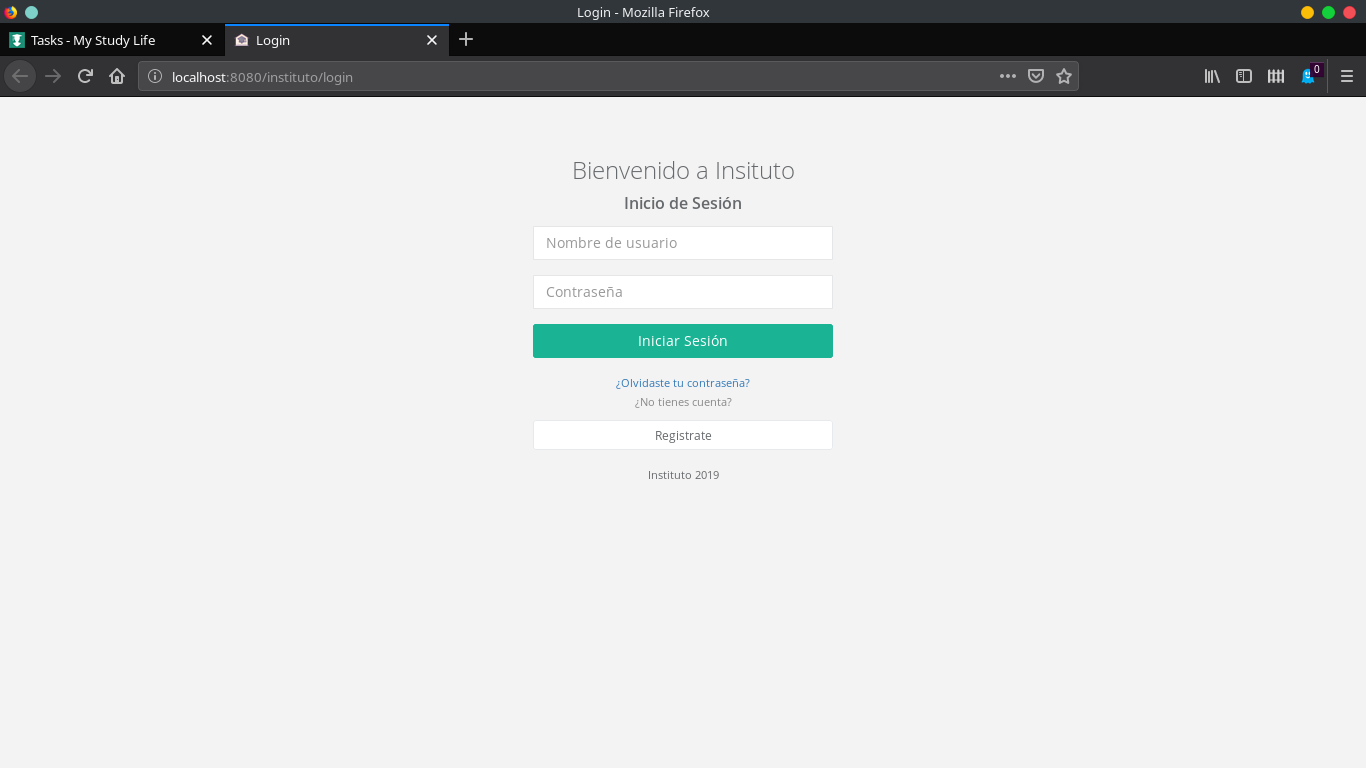
\includegraphics[width=\textwidth]{login.png}
 \caption{Login}
 \label{fig:login}
\end{center}
\end{figure}

\begin{figure}[H]
\begin{center}
 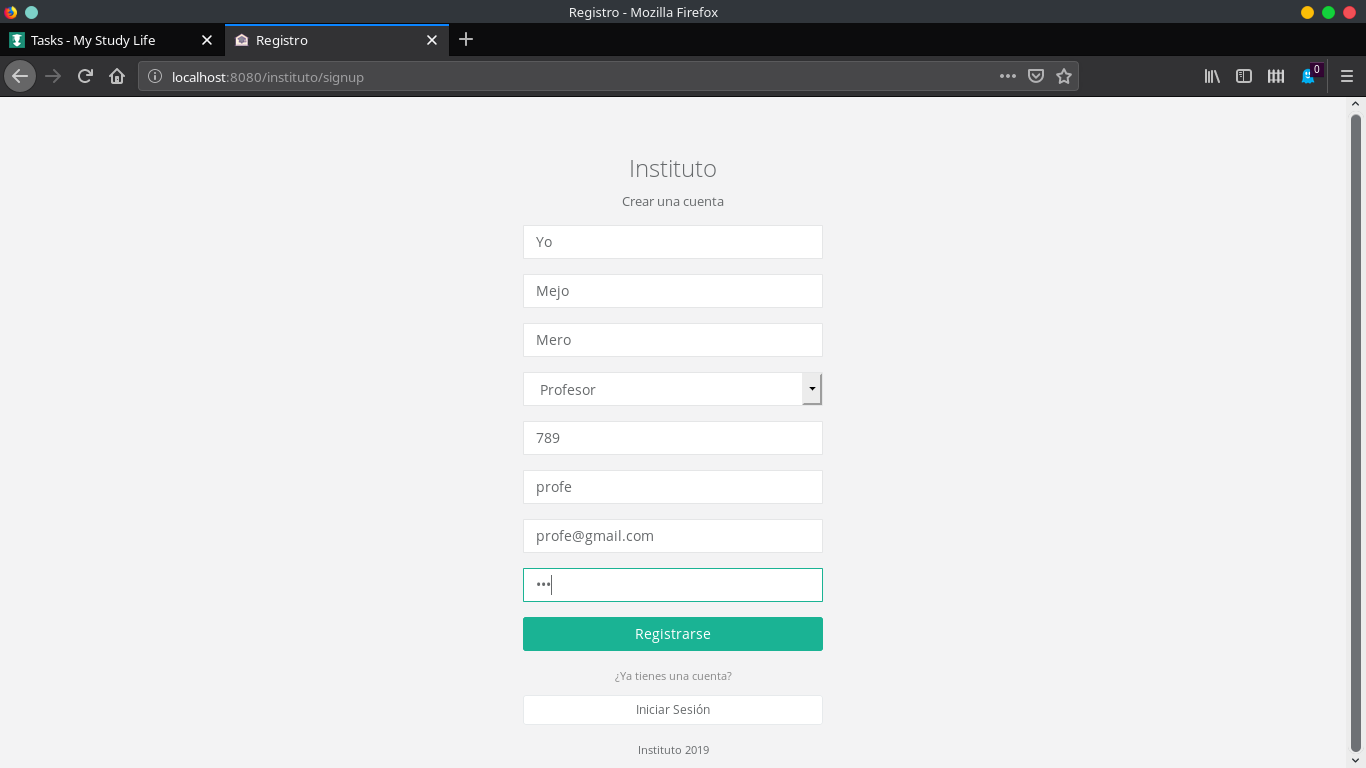
\includegraphics[width=\textwidth]{crear.png}
 \caption{Crear Cuenta}
 \label{fig:crear}
\end{center}
\end{figure}

\begin{figure}[H]
\begin{center}
 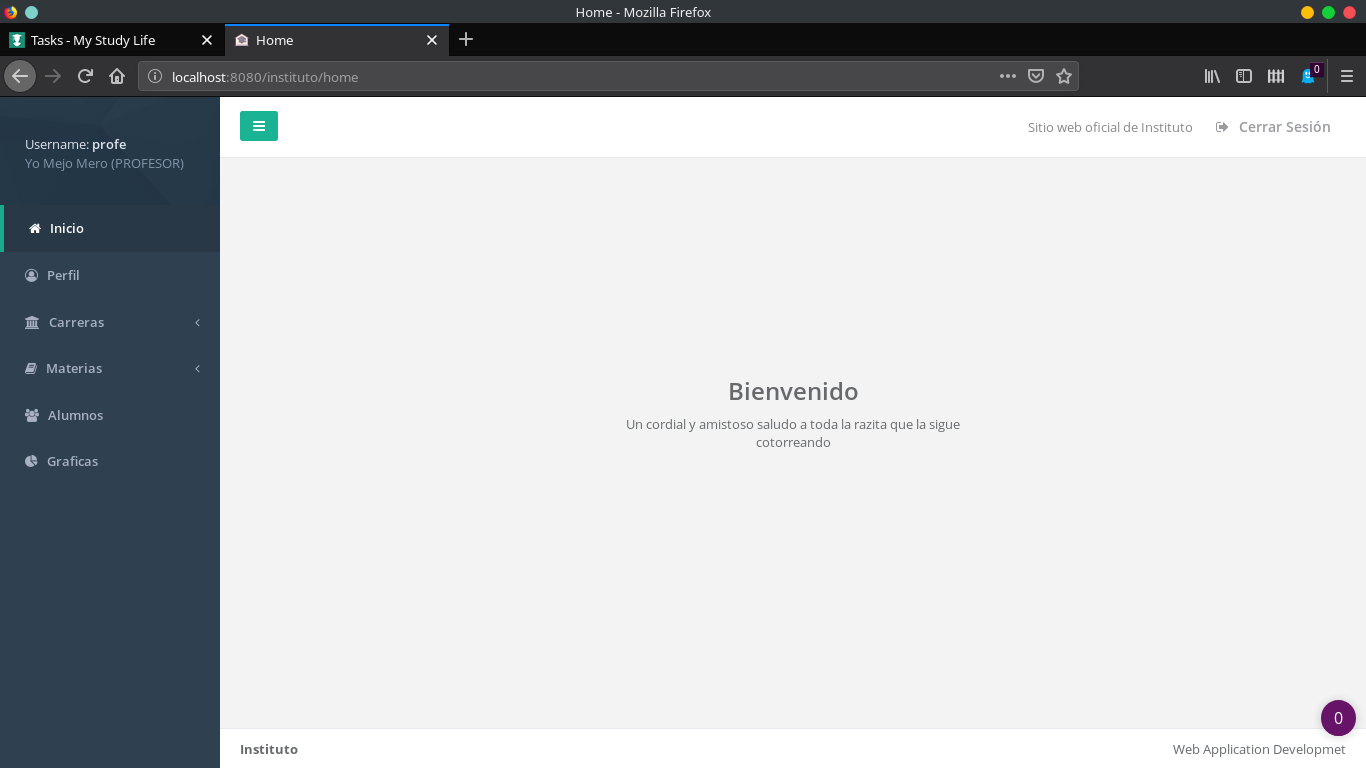
\includegraphics[width=\textwidth]{home.png}
 \caption{Home}
 \label{fig:home}
\end{center}
\end{figure}

\begin{figure}[H]
\begin{center}
 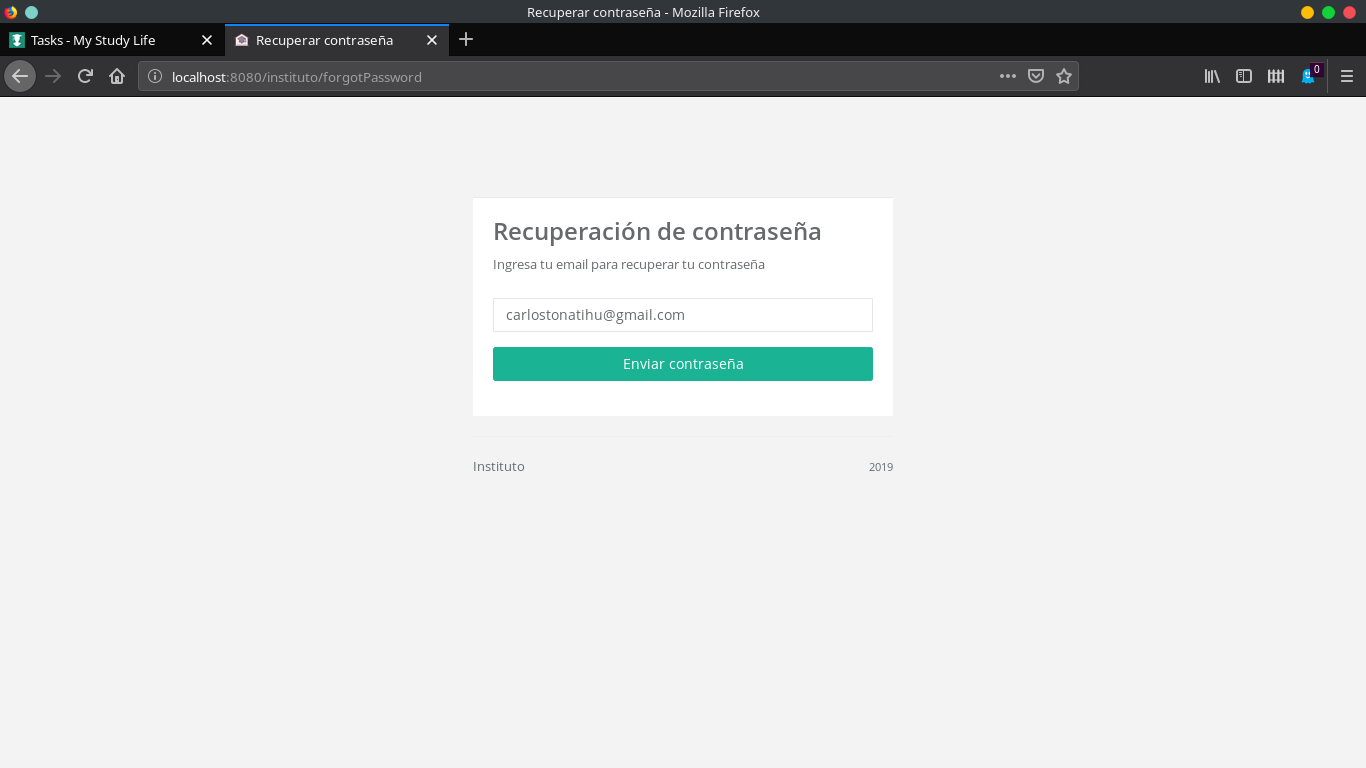
\includegraphics[width=\textwidth]{recuperar.png}
 \caption{Recuperar contraseña}
 \label{fig:recuperar}
\end{center}
\end{figure}

\begin{figure}[H]
\begin{center}
 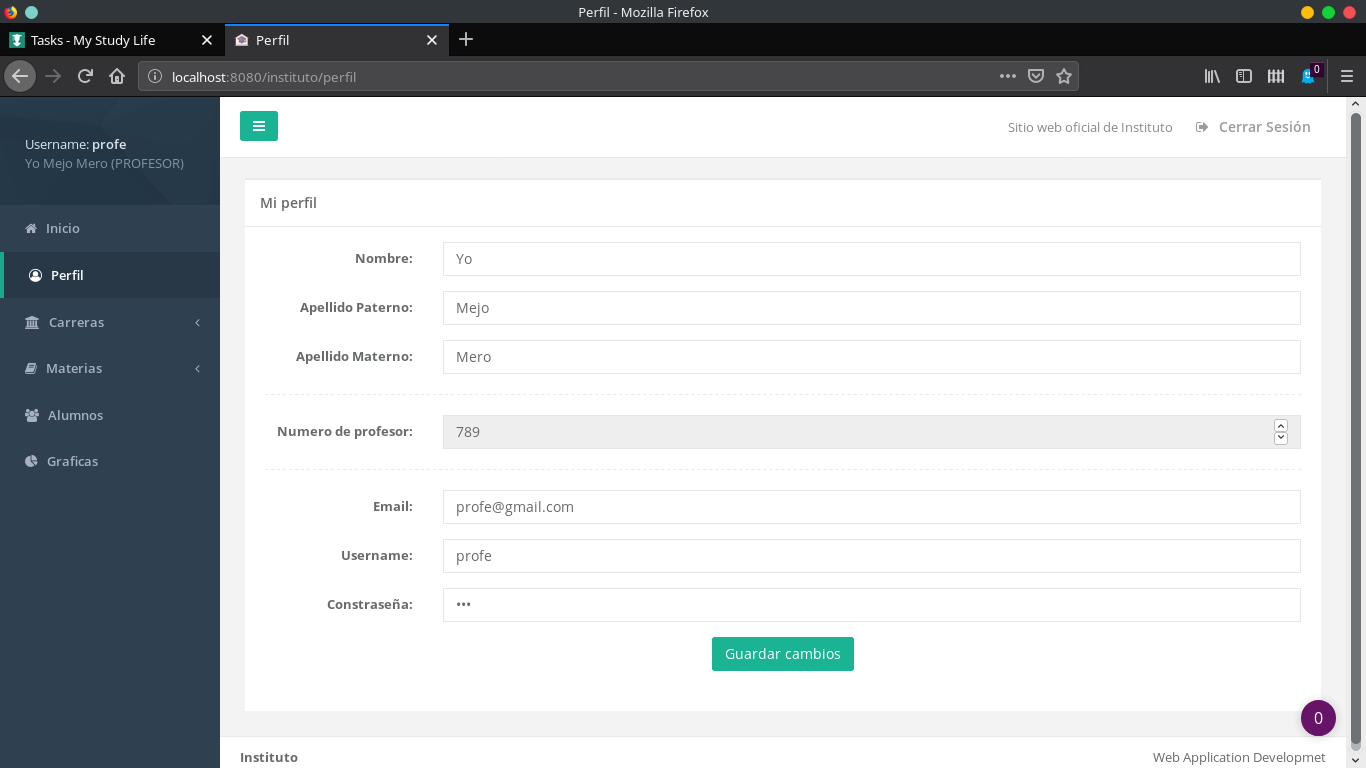
\includegraphics[width=\textwidth]{perfil.png}
 \caption{Perfil}
 \label{fig:perfil}
\end{center}
\end{figure}

\begin{figure}[H]
\begin{center}
 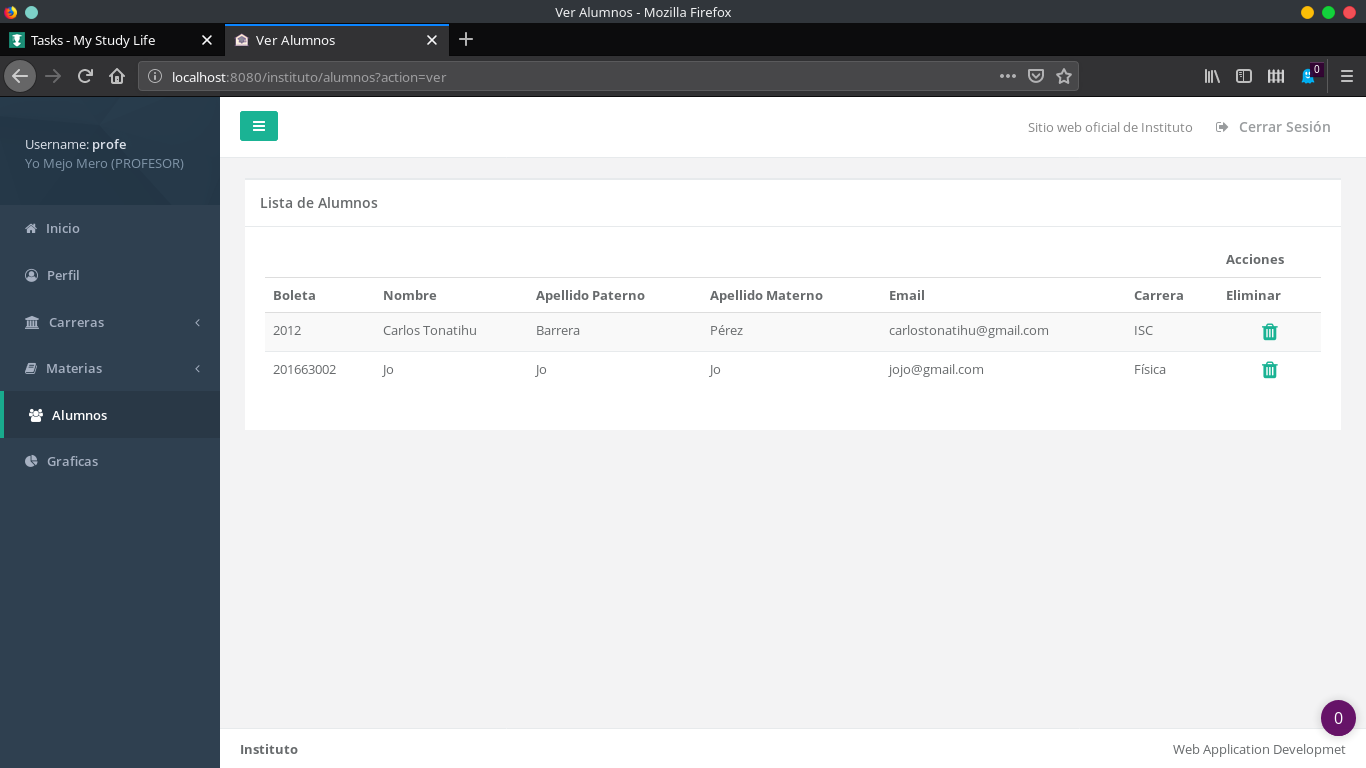
\includegraphics[width=\textwidth]{alumnos.png}
 \caption{Alumnos}
 \label{fig:alumnos}
\end{center}
\end{figure}

\begin{figure}[H]
\begin{center}
 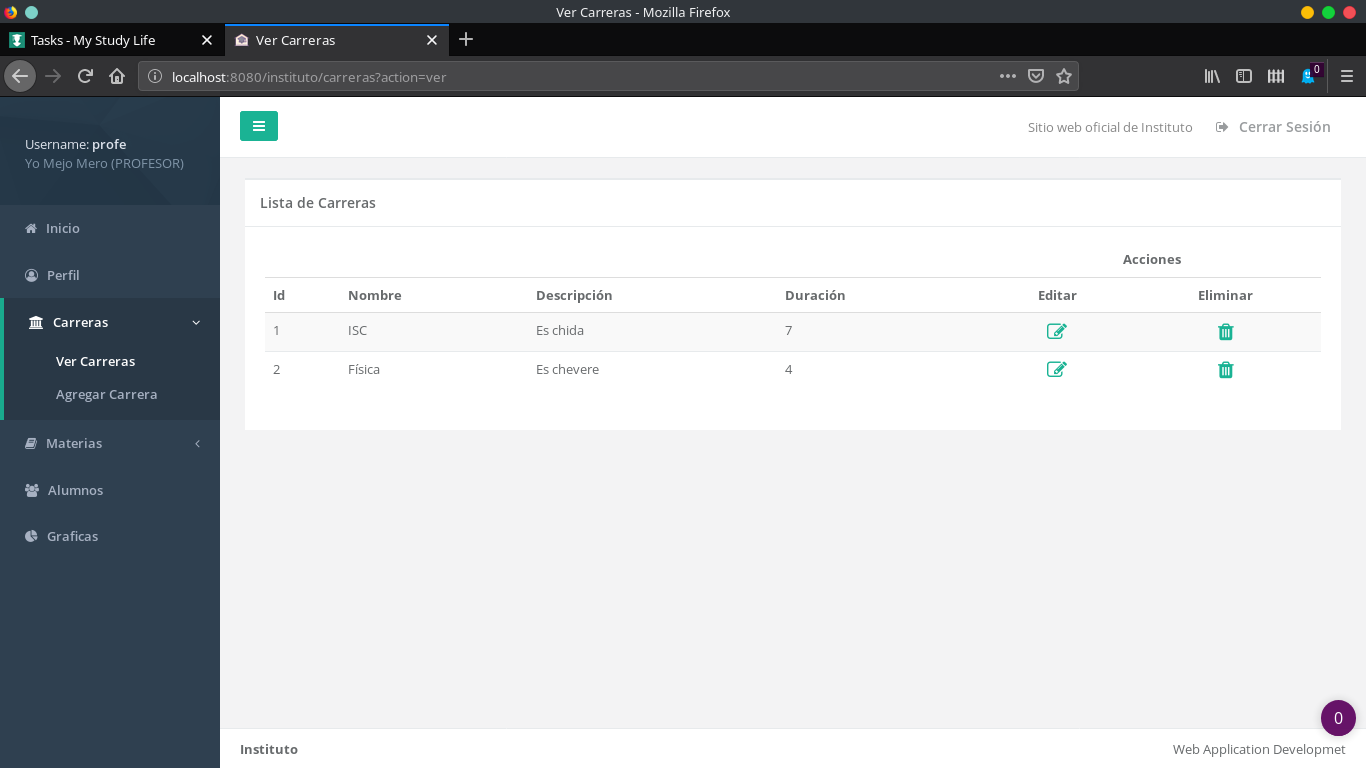
\includegraphics[width=\textwidth]{carreas.png}
 \caption{Ver carreras}
 \label{fig:carreas}
\end{center}
\end{figure}

\begin{figure}[H]
\begin{center}
 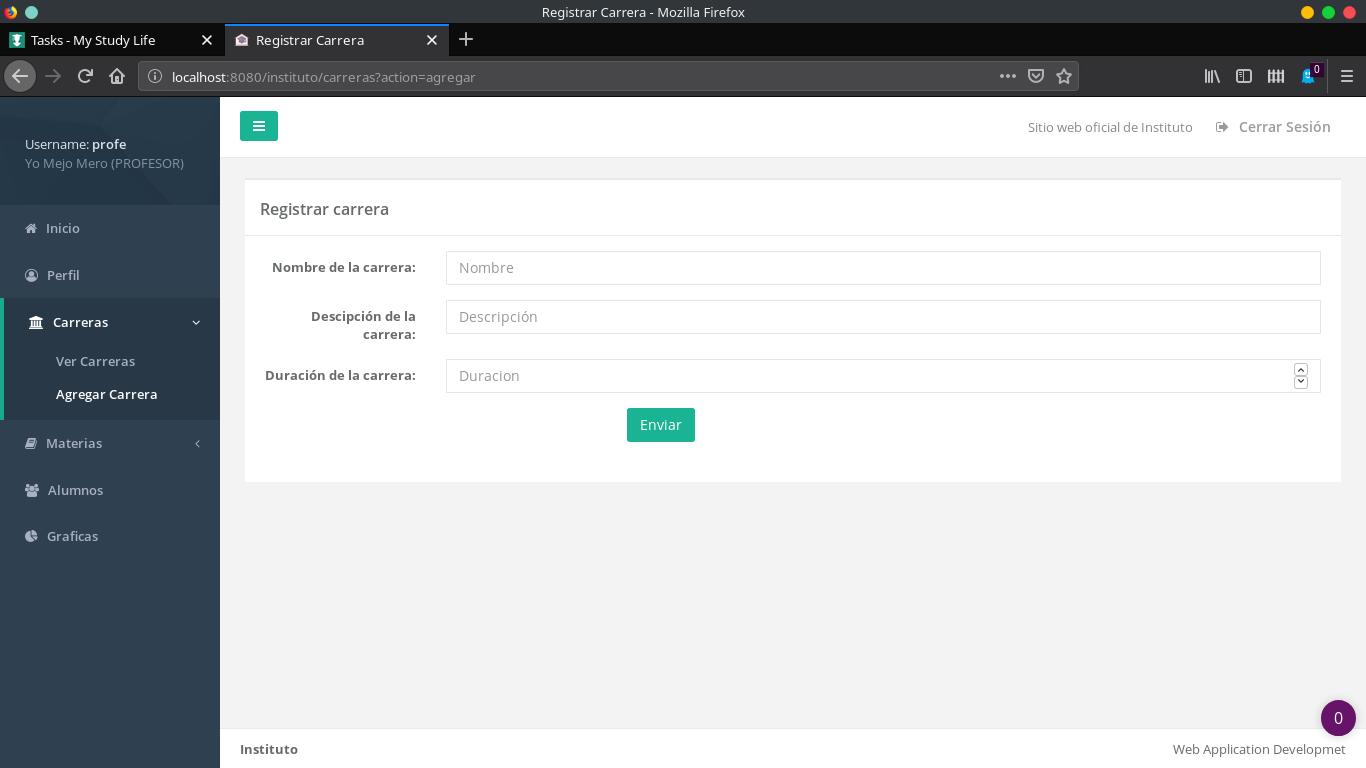
\includegraphics[width=\textwidth]{agregar_carrera.png}
 \caption{Agregar Carrera}
 \label{fig:agregar_carrera}
\end{center}
\end{figure}

\begin{figure}[H]
\begin{center}
 
\includegraphics[width=10cm]{contra.png}
 \caption{Correo de recuperación de contraseña}
 \label{fig:contra}
\end{center}
\end{figure}

\begin{figure}[H]
\begin{center}
 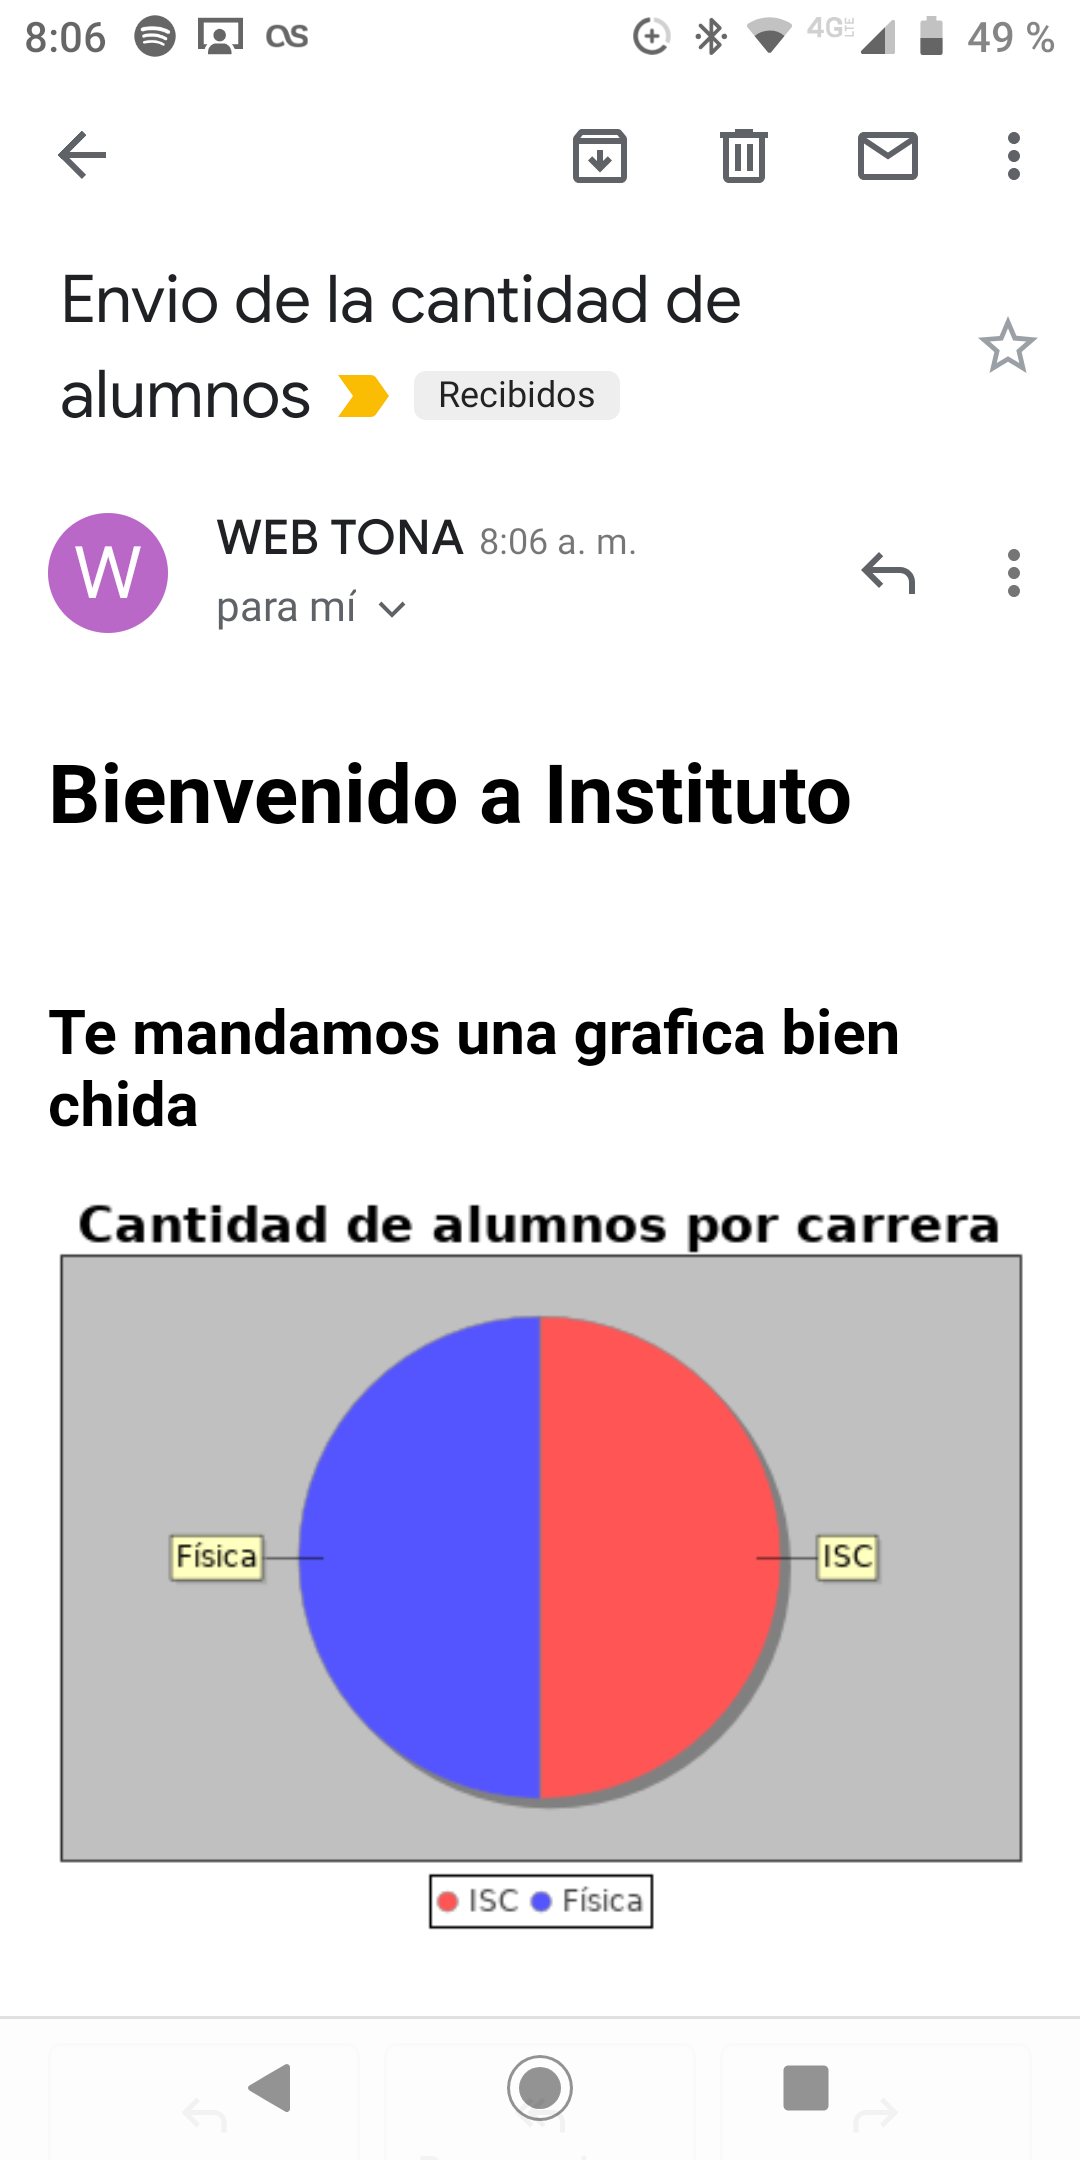
\includegraphics[width=10cm]{envio.png}
 \caption{Correo de envió de gráficas}
 \label{fig:envio}
\end{center}
\end{figure}
\section{Conclusiones}
Esta practica resulto difícil en un inicio debido a la nueva funcionalidad de 
envío de correos y generación de gráficas. Sin embargo, después de que se 
investigo un poco al respecto se pudo lograr el objetivo que se planteo en un 
inicio. Así que en un futuro la implementación de este tipo de características 
sera más sencillo de hacer, he incluso se puede mejorar.

\end{document}
